\section{Problèmes au cours du projet}

Dans un premier temps, nous avons créé des premières pages HTML afin d'avoir un rendu visuel et de définir un premier style CSS servant à voir, pour le développement, à quoi s'apparenterait les pages finales.

\begin{figure}[H]
    \begin{center}
	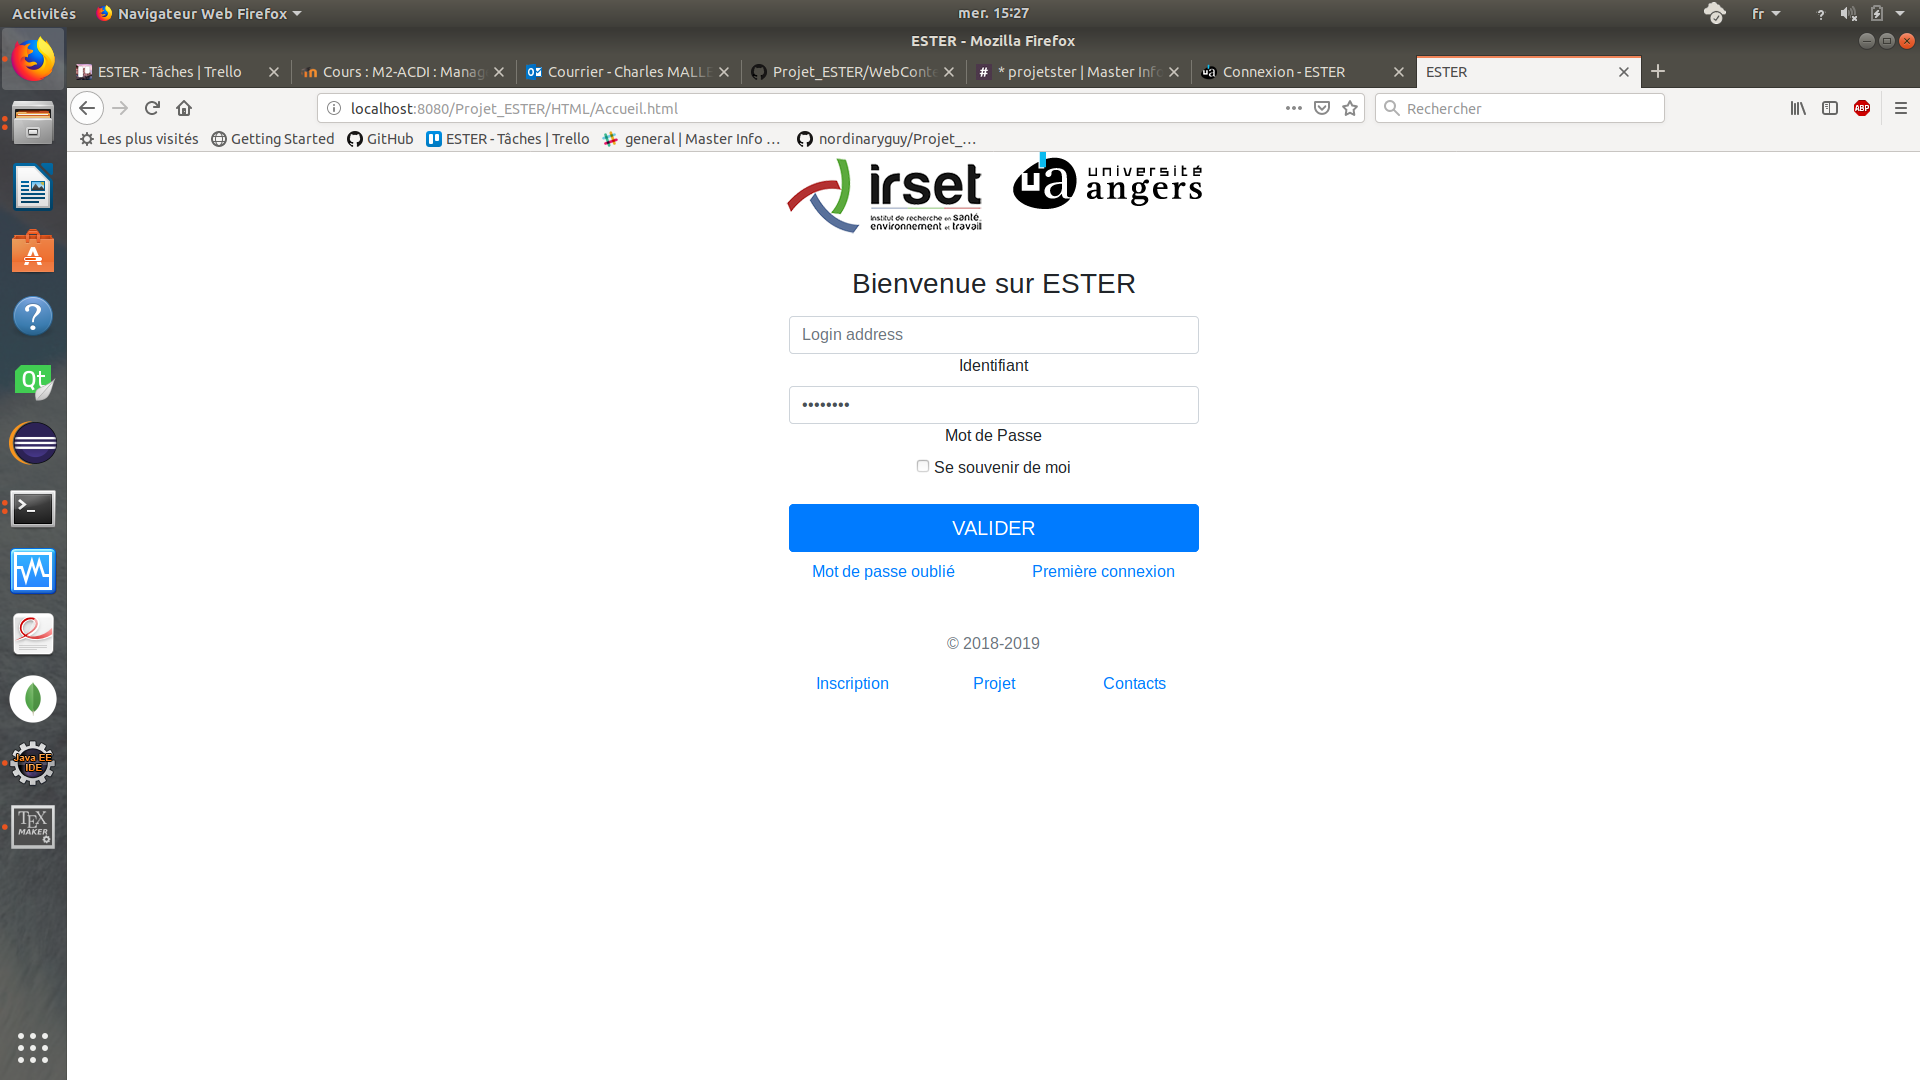
\includegraphics[scale=0.2,trim=4cm 0cm 4cm 5.3cm, clip=true]{img/OldConnexion}
    \end{center}
    \caption{Ancienne Page de Connexion}
\end{figure}

\begin{figure}[H]
    \begin{center}
	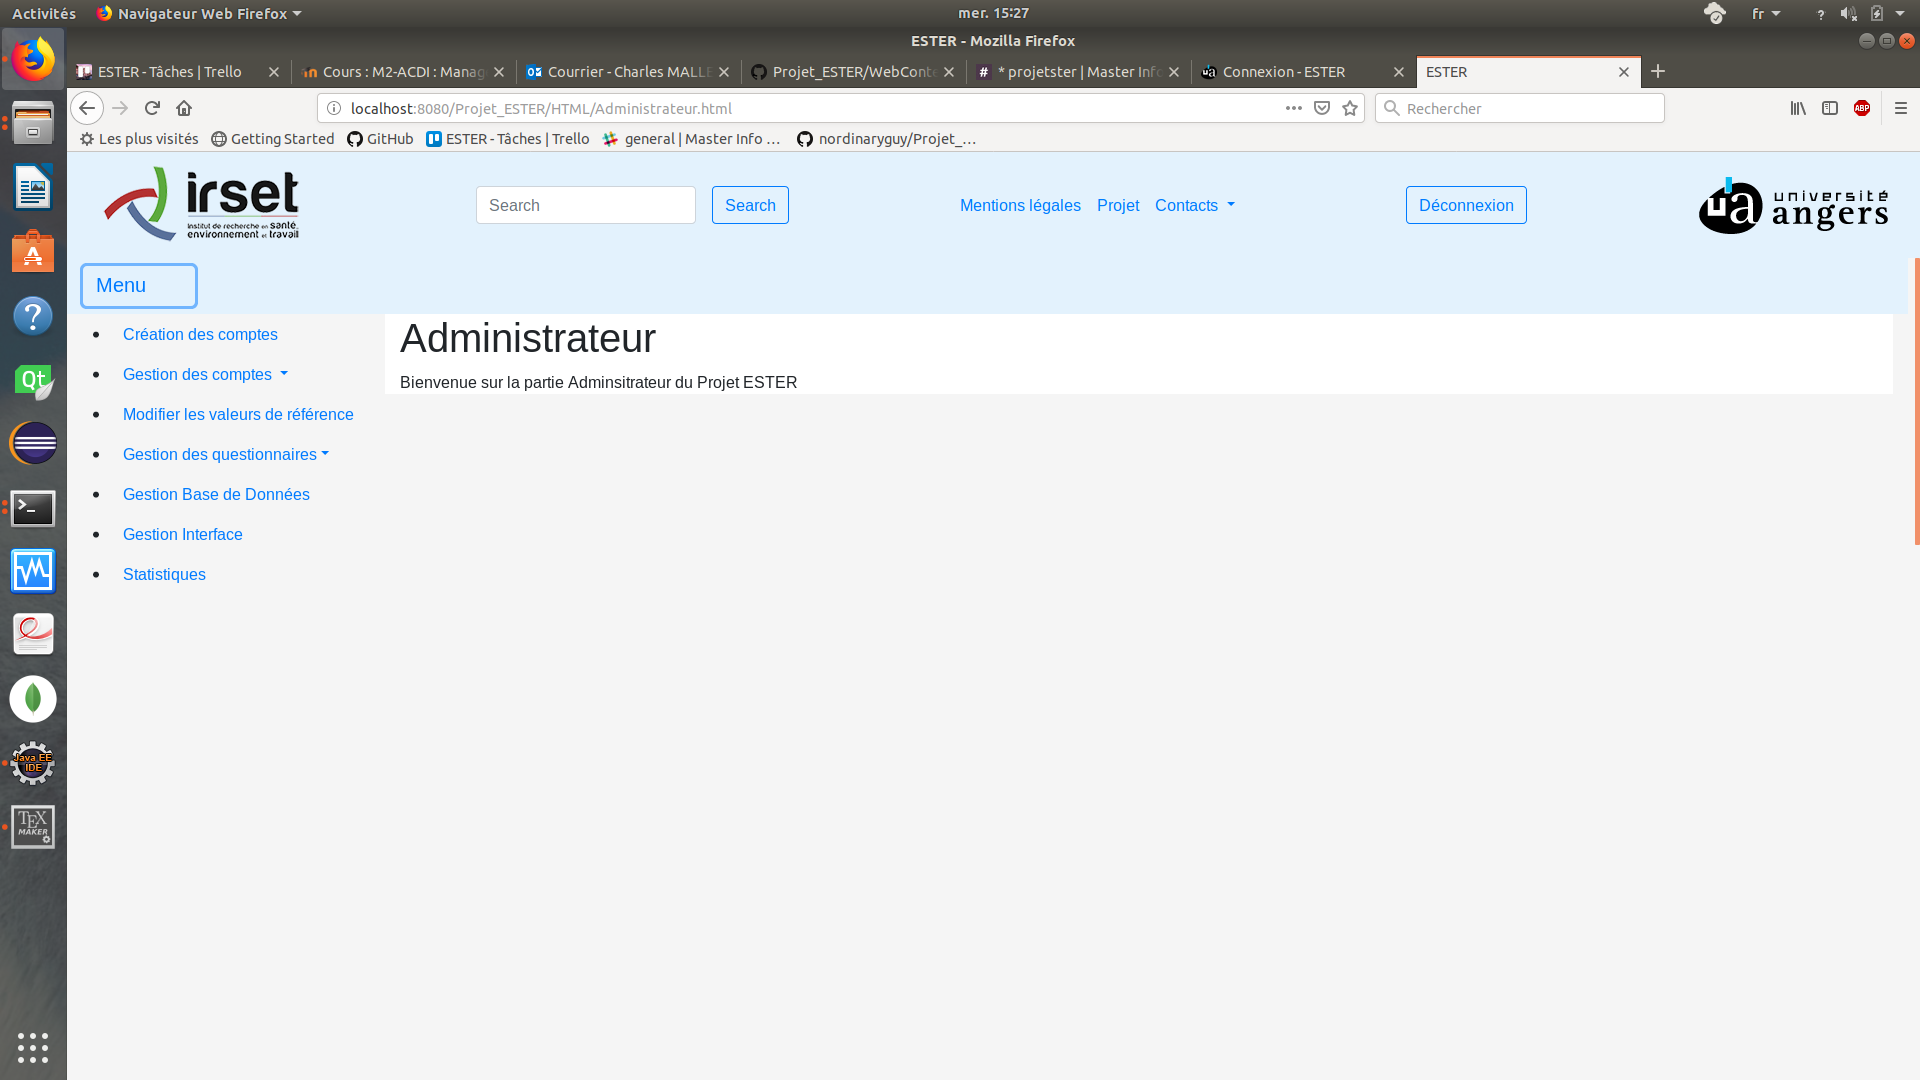
\includegraphics[scale=0.2,trim=2.8cm 0cm 0.8cm 5.3cm, clip=true]{img/OldAdmin}
    \end{center}
    \caption{Ancienne Page de l'Administrateur}
\end{figure}

Toutefois, les scripts HTML ont fini remplacés par des scripts JSP car plus avantageux comme dit précédemment. D'un autre côté, nous n'avons pas tous défini de la même manière nos styles CSS. Ce fut les membres d'ESTER qui décidèrent en conséquence du visuel qu'ils préféraient. Une fois la réunion de novembre passée, nous avons appliqués les modifications désirées et directement réécrit dans des scripts JSP. Cependant, ces changements nous ont coûté un peu de temps qui aurait pu nous être utile dans l'implémentation d'autres fonctionnalités.


\section{Perspectives d'amélioration}

